

\documentclass{llncs}
%
\usepackage{makeidx}
\usepackage{graphicx}
\usepackage{url}
\usepackage{bookmark,hyperref}
\usepackage{ntheorem}
\usepackage{hyperref}
\usepackage{url}
\usepackage{graphicx}
\usepackage[usenames]{color}
\usepackage{enumerate}
\usepackage{pdfpages} 
\usepackage{listings}
\usepackage{lscape}
\usepackage{stmaryrd} 
\usepackage{indentfirst}
\usepackage{multirow}
\usepackage{color}
\usepackage{booktabs}
\usepackage{float}
\usepackage{longtable}
\usepackage[toc,page]{appendix}
\usepackage{amsmath}
\usepackage{amsfonts}
\usepackage{enumitem}
\usepackage{textcomp}
\usepackage{multirow}
\usepackage{subfigure}
\usepackage{gensymb}
\usepackage{epstopdf}
\usepackage{mathtools}
\usepackage{float}
\usepackage{sidecap}
\usepackage{textcomp}
\usepackage{pgfplots}

%%%%%%%%%%%%%%%%%%%%%%%%%%%%%

\begin{document}
	
\title{Kinect and IMU sensors imprecisions compensation method for human limbs tracking}
	
\titlerunning{Kinect and IMU characteristics}  
	
\author{Grzegorz Glonek \and Adam Wojciechowski}
	
\authorrunning{Grzegorz Glonek \and Adam Wojciechowski}  
	
\tocauthor{Grzegorz Glonek, Adam Wojciechowski}

\institute{Institute of Computer Science\\Lodz University of Technology, Lodz, Poland,\\
	\email{grzegorz@glonek.net.pl},
	\email{adam.wojciechowski@p.lodz.pl}}
	
\maketitle            
\begin{abstract}
	Microsoft Kinect v.1 and inertial measurement units (IMU) became very popular and broadly available depth and inertia estimating devices, which allow home users to detect and track human limbs motion. Due to their working characteristics both of these devices are sufficient for casual scenarios, where precision is not a crucial factor. In the following paper a detailed review of their characteristics, verified by experiments of both devices, is presented, as well as the method of their imprecisions compensation. Comparing with other authors, the obtained limbs tracking accuracy improvement (by 12\%) has proved that elaborated method outperforms other solutions. 
\end{abstract}
	
\section{Introduction}
Since Microsoft Kinect has been released in 2010 and inertial devices have become an integral and almost mandatory part of every smartphone, motion tracking and motion detection became very popular and easily available for the home usage. Kinect is mainly used in the field that it was created for games and entertainment. However, due to the limitations, mostly caused by the way it was built, only relatively simple casual games were developed for this controller. On the other hand, Microsoft Kinect became a popular subject for researchers, who want to find out how this device might be applied in more advanced scenarios \cite{Lange2012,Chang2011}. 

The second of the mentioned devices -- inertial measurement unit (IMU) -- can be easily found in almost every modern smartphone. From home user's point of view, the most noticeable functionality, implemented thanks to these devices, is a screen view rotation. Also applications that measure number of pedestrian's steps base on them \cite{Jayalath2013,walklogger}. Of course, these devices also have some flaws and limitations that need to be taken into consideration in order to achieve accurate and stable results.

Mentioned controllers data fusion methods were also studied as to increase tracking performance compensating relative devices imprecisions  \cite{Bo2011,Destelle2014,Murray-Smith2014,Kalkbrenner2014}. Nevertheless authors have concentrated mostly on different types of Kalman filter raw data fusion rather then devices inherent characteristics correction. 

Basing on self experiments as well as on existing publications, presented paper describes thorough characteristics of both devices and propose a new method compensating their major imperfections and limits. Suggested method focuses on individual devices as well as on their fusion, what allows to compensate incompleteness of information that both types devices have.
%In further part of this article measurement and working characteristics of both devices have been described, as well as a proposed method of their limitations compensation.

%==================================================================================	
\section{Kinect characteristics}
Microsoft Kinect version 1 is an RGB-D camera built from two CMOS cameras and integrated infrared (IR) projector. One of these CMOS is responsible for an RGB signal and the second one is calibrated to record IR beam's view. However, the most important part is the main chip created by PrimeSense company, which is responsible for the body motion tracking and the body gesture recognition. The simplified device schema is presented in figure \ref{fig:characteristics:kinect:inside}.

According to the official specification, an operation range of Kinect is between  $0.8m$ and $4m$ in the field of view $57\degree$ horizontally (static) and $43\degree$ vertically. The specification doesn't include any information on the possible variety of measurements accuracy in this area. The range defined in the official specification is presented in figure \ref{fig:characteristics:kinect:range}. However, some users \cite{stack:kinect2011} and researchers \cite{DiFilippo2015} reported that different device series have a slightly different ranges where they operate, so above values should be treated as an average.

An important characteristic of Microsoft Kinect -- object distance measurement -- is directly related to the device design and used algorithm that bases on a structured light idea. Microsoft hasn't published any document describing how the algorithm actually works, but basing on original patent forms \cite{patent:20080106746,patent:20100020078,patent:20100118123} and independent research, some rough description can be created \cite{reichinger2011}, as well as an image of the used light pattern (1 out of 9 repeatable sub-patterns is presented in fig. \ref{fig:characteristics:kinect:dotPattern}).
Basing on the image of a structurally lighted scene, Kinect analyses the distortion of IR dots pattern to estimate objects' distance. Two techniques are used in parallel to compute such estimation: \textit{dots blurriness analysis} and \textit{stereo-vision based on a single IR camera and a projector}. A detailed description of both techniques can be found in  \cite{Rzeszotarski2006,Fofi2004}.

A human skeleton estimation is based on the previously estimated depth map and pattern recognition built on about 100 000 predefined samples. Pose classification process bases mostly on machine learning and random decision forest as well as some object detection algorithms i.e. Viola-Jones\cite{Shotton2008,Shotton2011}. It is worth noticing that a signal recorded from an RGB camera is not used at all in the human skeleton estimation process.

\begin{figure}[h!]
	\centering 
	\begin{minipage}[b]{0.49\linewidth}
		\centering
		\vspace{2.5cm}
		%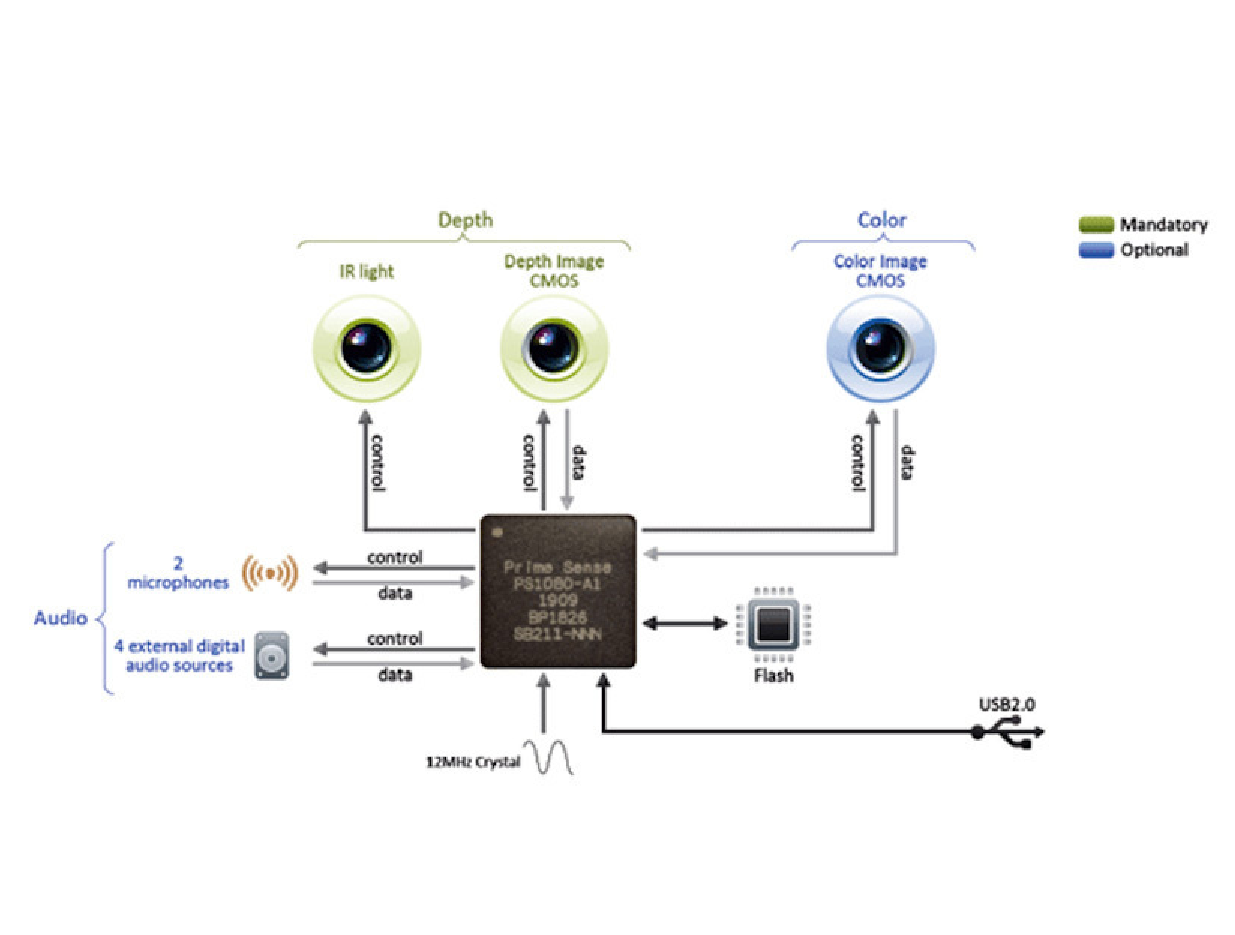
\includegraphics[width=\textwidth]{Images/Fig01}%{Images/kinectSchema}
		\caption[]{Simplified Microsoft Kinect v.1 controller build schema \cite{kinectFixit2016}}
		\label{fig:characteristics:kinect:inside} 
	\end{minipage}
	\begin{minipage}[b]{0.49\linewidth}
		\centering 
		\vspace{2.5cm}
		%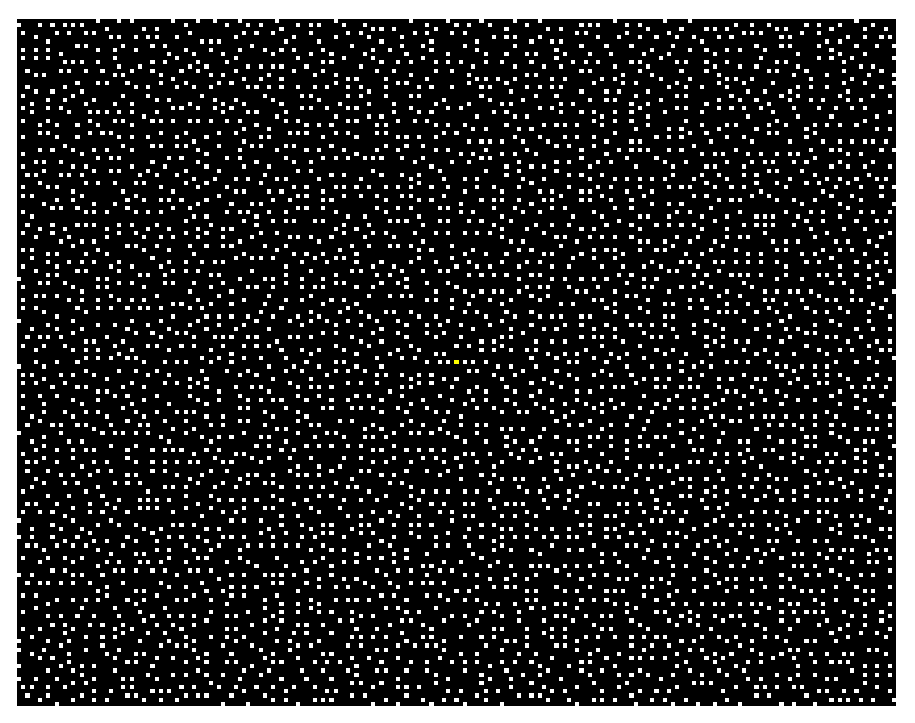
\includegraphics[width=\textwidth]{Images/Fig02}%{Images/kinect-pattern_3x3}
		\caption[]{Repeatable sub-pattern of IR scene lighting structure\cite{reichinger2011}}
		\label{fig:characteristics:kinect:dotPattern}
	\end{minipage}
\end{figure}
		
\begin{figure}[h!] %Fig03
	\centering
	\subfigure[Horizontal range]
	{
		%	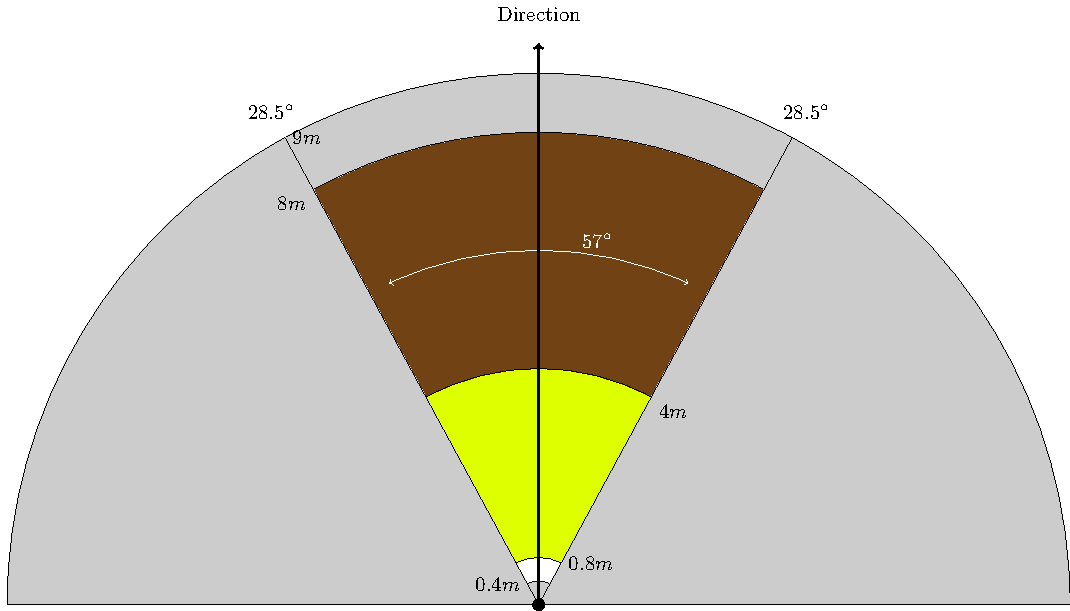
\includegraphics[scale=0.4]{Images/Fig03a.pdf}
			\vspace{2.5cm}	
	}
	\subfigure[Vertical range]
	{
		%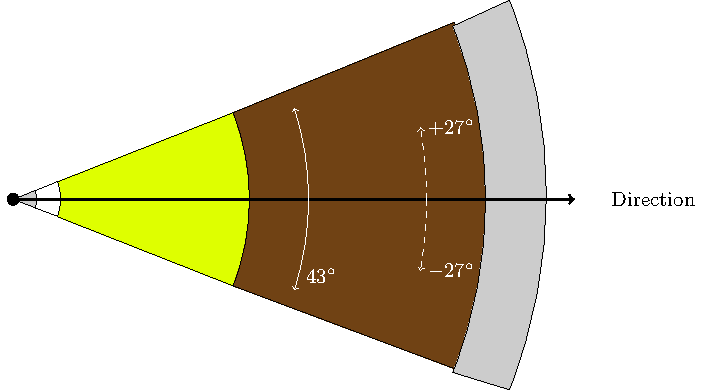
\includegraphics[scale=0.5]{Images/Fig03b.pdf}
		\vspace{2.5cm}	
	}
	\subfigure{
		%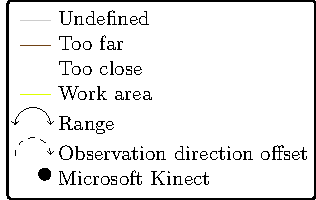
\includegraphics[scale=0.6]{Images/Fig03c.pdf}
			\vspace{2.5cm}	
	}
	\caption{Microsoft Kinect v.1 work range}
	\label{fig:characteristics:kinect:range}
\end{figure}
		
		
%\subsection{Limitations}
One of the basic limitations of this device is the sun light sensitivity. Scene depth estimation relies on the IR light, whereas the sun light contains a full colours spectrum in both, visible and an invisible range. This causes a noise in the light pattern. The great example of the sun light impact on measurements can be found in \cite{Suarez2012}. That makes Kinect useless in outdoor scenarios and makes it difficult to use two or more Kinects simultaneously. However, despite Microsoft recommendation to not use multiple Kinect controllers in one room, scientists worked on and published methods on combining signals from several devices \cite{Kitsikidis2011,Asteriadis2013,Schroder2011}.

Other significant limitation is related to completeness of information gathered from the device. An inherent skeleton estimation algorithm retrieves positions of 20 joints and rotations of bones between these joints. However, every joint is reduced to a single point and bones rotations are estimated basing on these points, what results in the lack of information about rotation along the bone (roll).

Two other limitations: occlusions and variety of the depth measurements accuracy in the field of observation, are treated also as significant. The first one occurs when a part of user's body is covered by another object or is hidden behind any other body part (self-occlusion). When the occlusion happens, Kinect tries to estimate the location of the covered joint or stops tracking it, when it is not able to provide any rough estimation. The occlusion by an external object seems to be intuitive and doesn't require any additional explanation, but self-occlusion is connected with Kinect's sensitivity to user's rotation to the camera. The official specification mentions that Kinect is designed to work in a \textit{face off pose}. However, this document doesn't define what \textit{face off} means and what is the exact angle between the human and the device when the occlusion occurs. Self experiments allow to observe how measurements change when the user rotates in front of the camera. The angle $\alpha$ (fig. \ref{fig:characteristics:kinect:bodyRotationAngle}) represents such a rotation and has been calculated with eq. \eqref{eq:characteristics:kinect:bodyRotationAngle}. It is also worth to mention that each joint can be in any of 3 tracking states:
\begin{itemize}
	\item \textsl{Tracked} -- set for fully visible, not noised joint with directly measured position.
	\item \textsl{Interfered} -- joint which position can be estimated but not measured.
	\item \textsl{NotTracked} -- joint which position cannot be measured nor estimated.
\end{itemize}

Occluded joints can be in \textsl{Interfered} or \textsl{NotTracked} state.

\begin{figure}[h!]		
	\centering
	%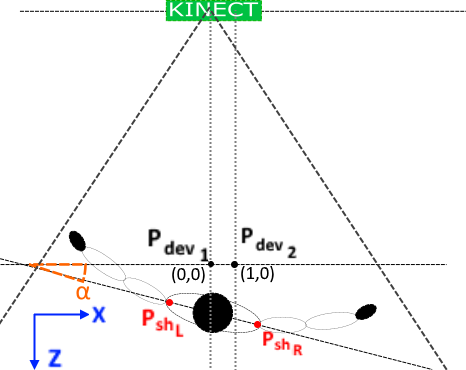
\includegraphics[width=0.4\textwidth]{images/Fig04}%{images/kinectAngle}
	\vspace{2.5cm}
	\caption{Rotation angle $\alpha$ between user and Kinect}
	\label{fig:characteristics:kinect:bodyRotationAngle}
\end{figure}	

\begin{equation}   
	\label{eq:characteristics:kinect:bodyRotationAngle}
	\begin{split}
		&P_{Dev}.Z = P_{{Dev}_1}.Z - P_{{Dev}_2}.Z = 0 \\
		&P_{Dev}.X = P_{{Dev}_1}.X - P_{{Dev}_2}.X = -1 \\
		&P_{Sh}.Z = P_{{Sh}_L}.Z - P_{{Sh}_R}.Z \\
		&P_{Sh}.X = P_{{Sh}_L}.X - P_{{Sh}_R}.X \\
		\alpha &= 
		\begin{cases} 
			|atan(\frac{P_{Dev}.Z}{P_{Dev}.X}) - atan(\frac{P_{Sh}.Z}{P_{Sh}.X})| = atan(\frac{P_{Sh}.Z}{P_{Sh}.X}) & , P_{Sh}.X \neq 0 \\
			|atan(\frac{P_{Dev}.Z}{P_{Dev}.X}) - \frac{\Pi}{2})| = \frac{\Pi}{2}                                    & , P_{Sh}.X = 0    \\		
		\end{cases}
	\end{split}
\end{equation}
where:
\begin{itemize}
	\item $P_{{Dev}_1}.X, P_{{Dev}_1}.Z, P_{{Dev}_2}.X, P_{{Dev}_2}.Z$ -- X and Z axes coordinates of Kinect camera.
	\item $P_{{Sh}_L}.X, P_{{Sh}_L}.Z$ -- X and Z axes coordinates of user's left shoulder.
	\item $P_{{Sh}_R}.X, P_{{Sh}_R}.Z$ -- X and Z axes coordinates of user's right shoulder.
\end{itemize}

Charts form figures \ref{fig:characteristics:kinect:bodyRotationChart} and \ref{fig:characteristics:kinect:kinectRightHandElbowAngle} show measured joints tracking states and elbow angle changes during rotation respectively. All the time, observed joint has been visible to the camera and its angle hasn't changed (rotation in ''T-pose''). As we can see in fig. \ref{fig:characteristics:kinect:kinectRightHandElbowAngle}, when angle is greater than $50 \degree$ measurements turn to be unstable and unreliable.

\begin{figure}[h!]			
	\centering
		\subfigure[Joint tracking state]{\label{fig:characteristics:kinect:bodyRotationChart}
			%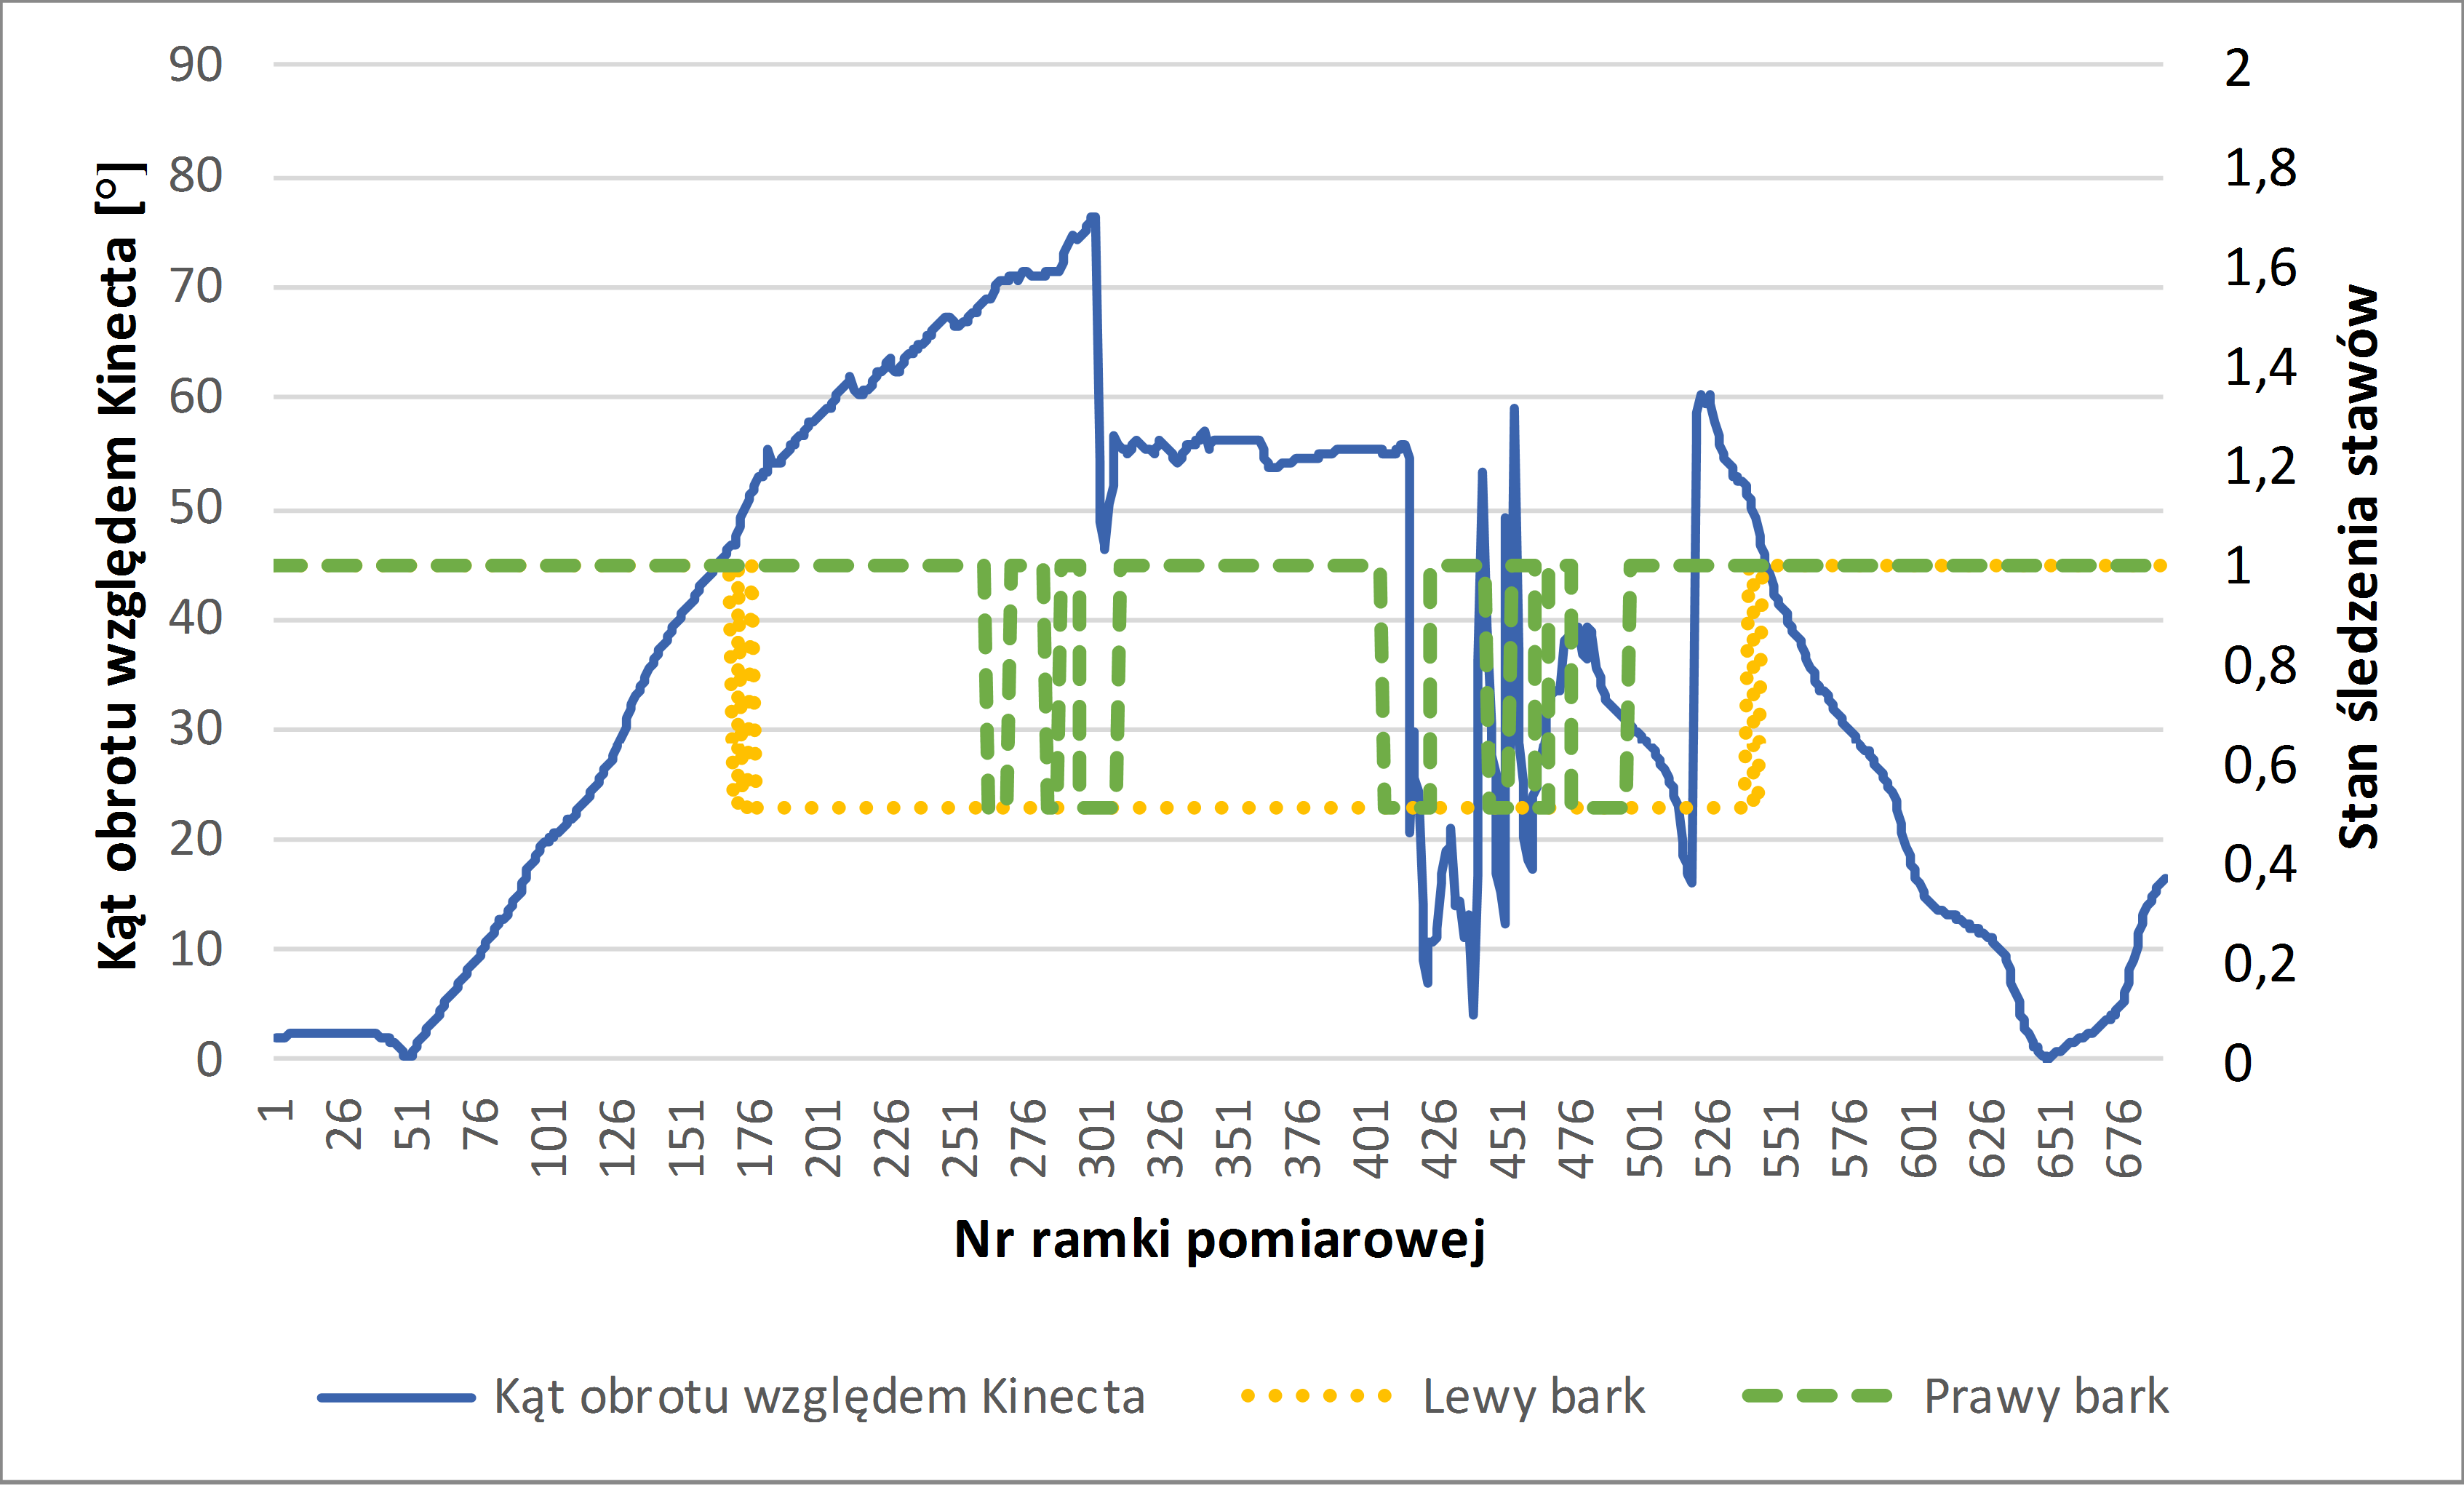
\includegraphics[width=0.45\textwidth]{images/Fig05a}%{images/kinectRotation}
			\vspace{2.5cm}
		}
		\subfigure[Right elbow angle]{\label{fig:characteristics:kinect:kinectRightHandElbowAngle}
			%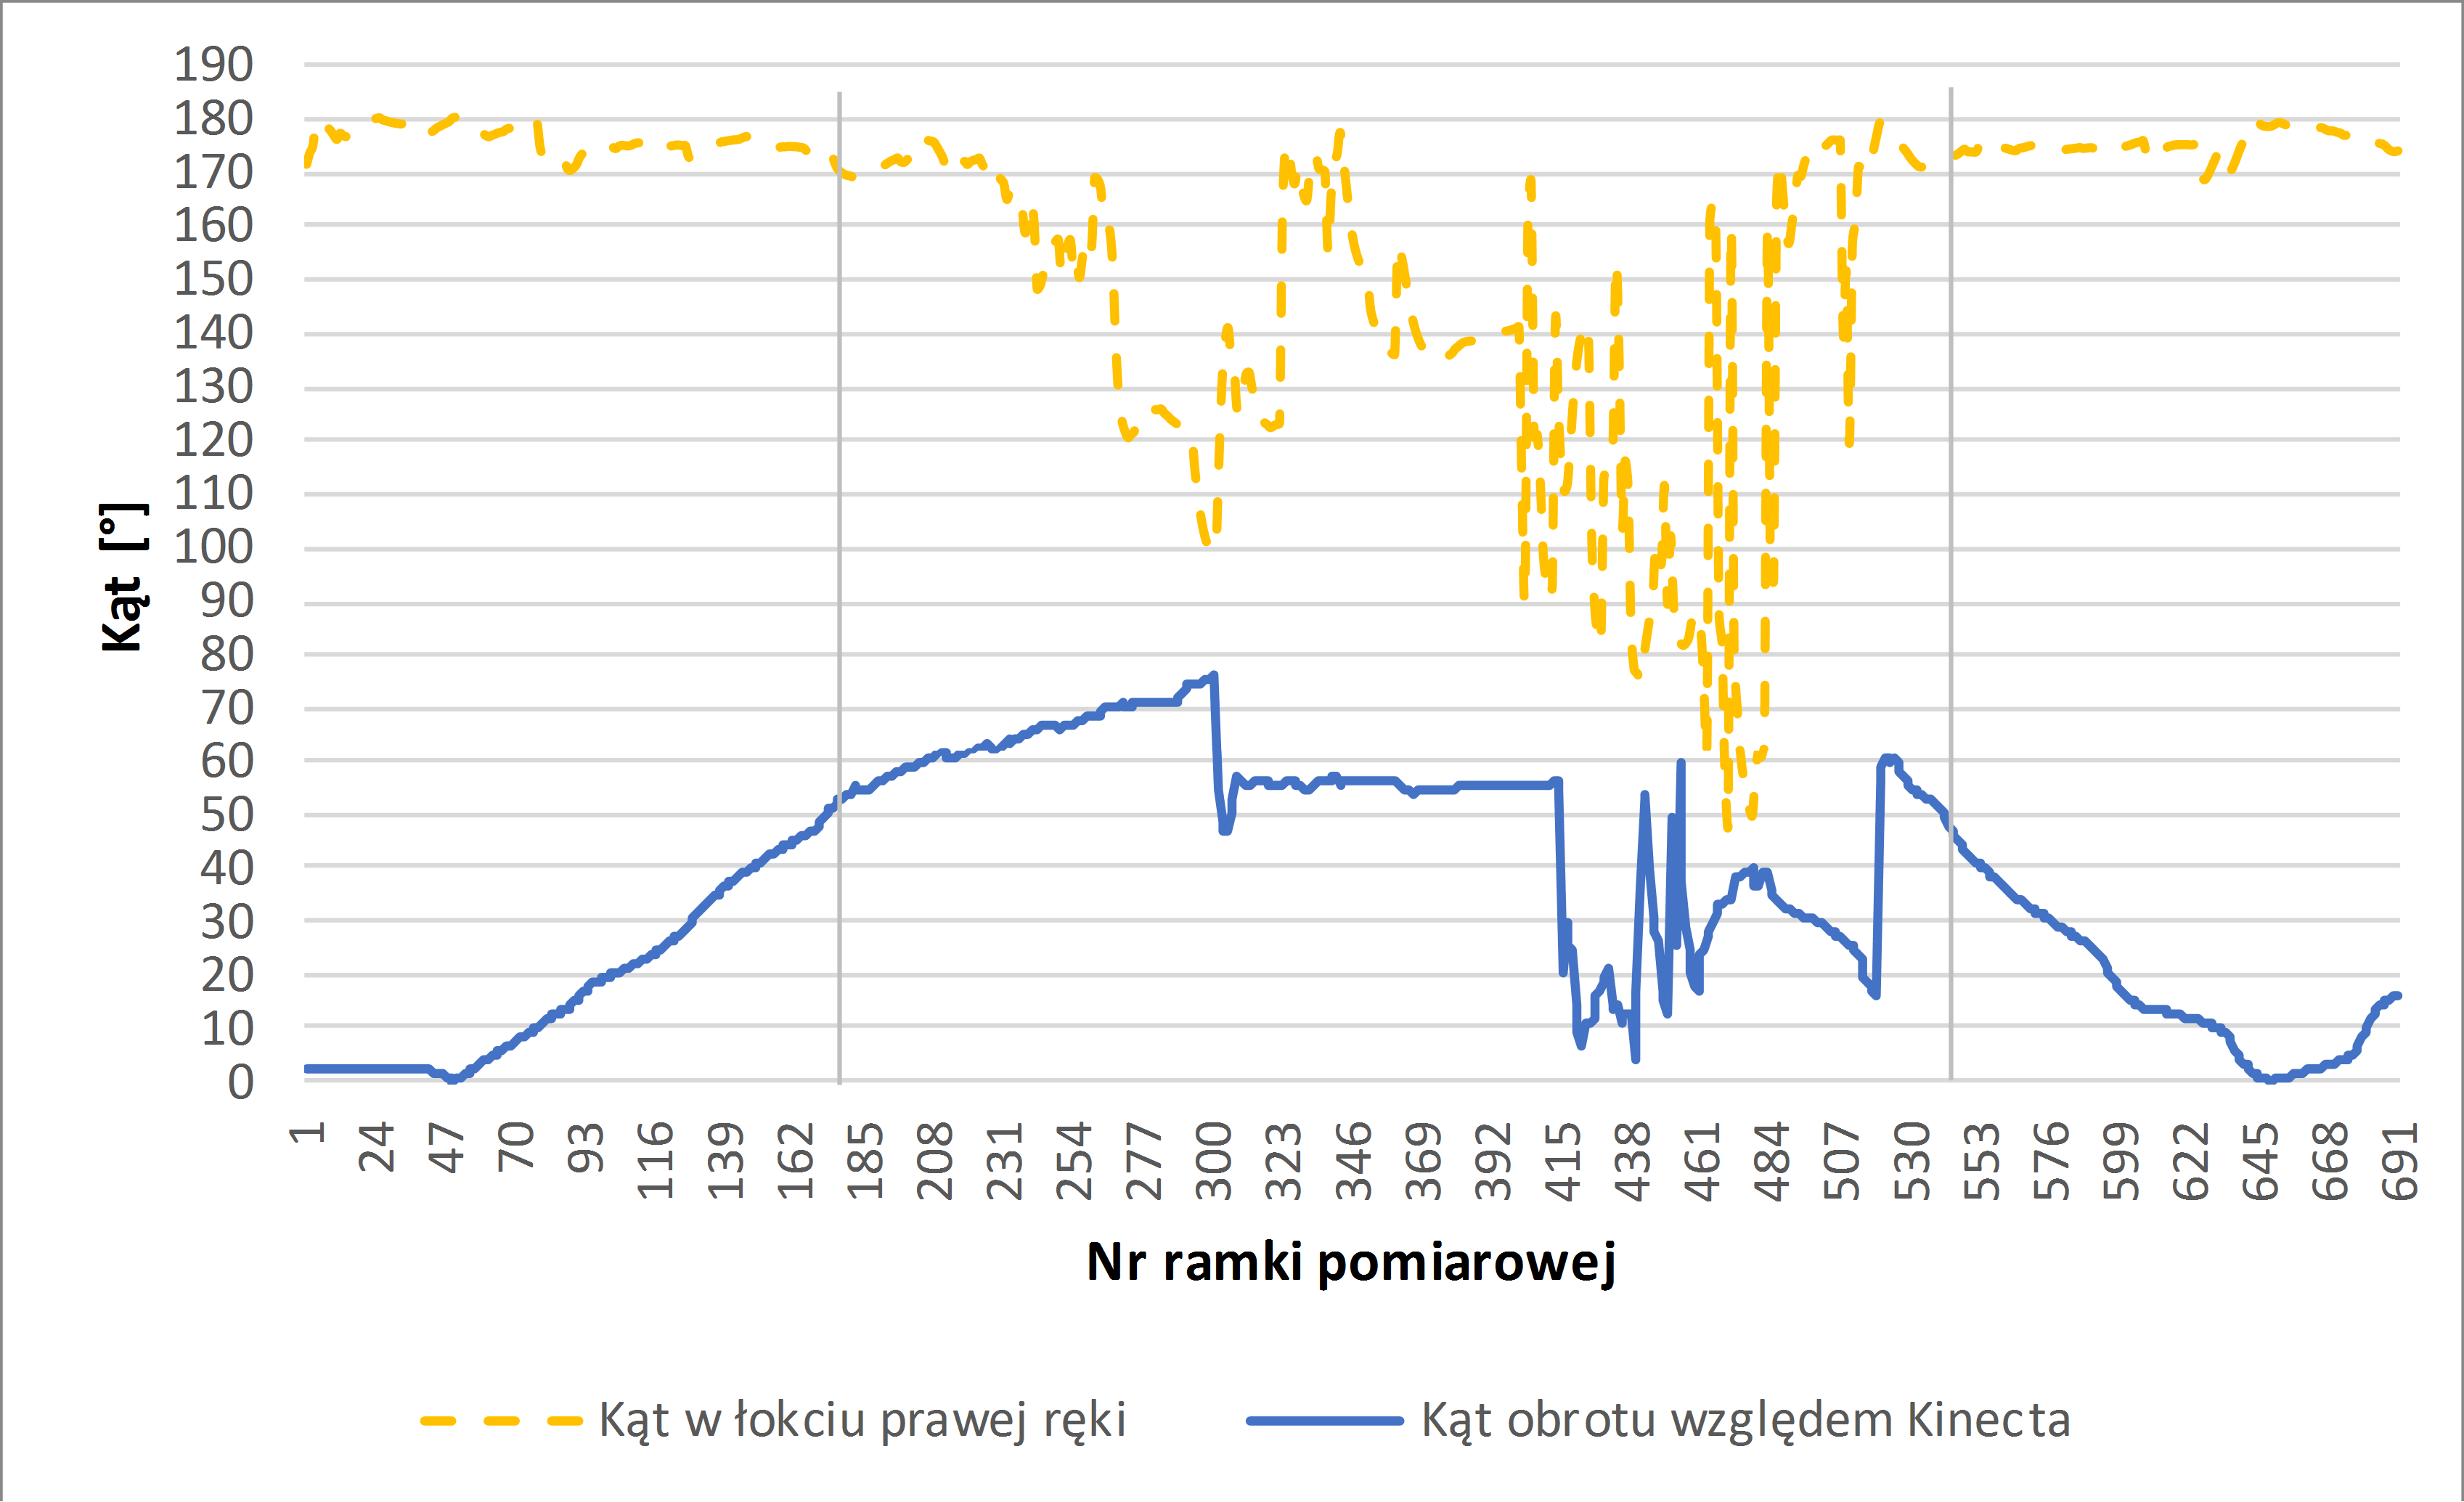
\includegraphics[width=0.45\textwidth]{images/Fig05b}%{images/kinectRightHandElbowAngle}
			\vspace{2.5cm}
		} 
		\subfigure[Orientation measurements standard deviation]{\label{fig:characteristics:imu:kinectRotationVariance}
			%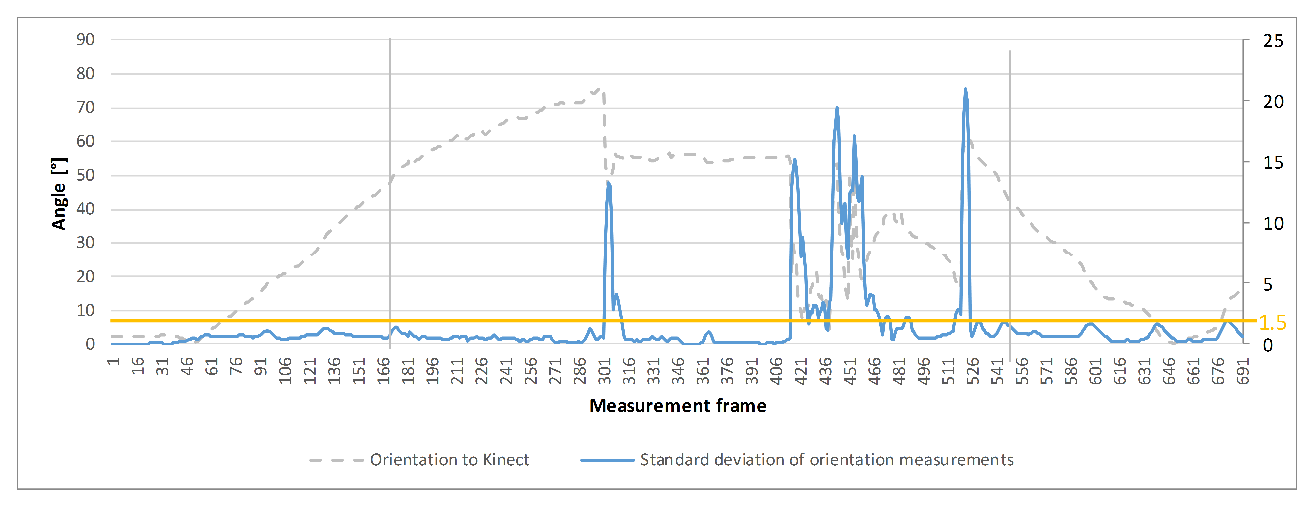
\includegraphics[width=0.75\textwidth]{images/Fig05c}%{images/kinectRotationVariance}
			\vspace{2.5cm}
		} 			
	\caption{Joints measurements reflecting user orientation changes in relation to the Kinect}
	\label{fig:characteristics:kinect:orientationCharts}
\end{figure}

Fluctuations in depth measurement accuracy have been observed in experiment with a professional Vicon Motion Capture system. During that experiment, the user had to move back in the distance from $0.8m$ to $4m$ from the camera and such distance has been measured by Kinect and Vicon simultaneously. The results show that in the close range Kinect slightly underestimates the distance and in the far range it overestimates it. The optimum is located at the distance of $2m$ -- $2.3m$ from the camera.  Basing on measured values, model function has been estimated as the 3rd order polynomial ($y = a_0 + a_1x + a_2x^2 + a_3x^3$) calculated according to eq. \eqref{eq:polynominal}.
		
\begin{equation}
	\begin{split}
		X = 	\begin{bmatrix}
		x_1^0&x_1^1&x_1^2&x_1^3\\			
		x_2^0&x_2^1&x_2^2&x_2^3\\
		x_3^0&x_3^1&x_3^2&x_3^3\\
		\dots\\
		x_n^0&x_n^1&x_n^2&x_n^3
		\end{bmatrix} ,
		A &= 	\begin{bmatrix}
		a_0\\a_1\\a_2\\a_3
		\end{bmatrix} ,
		Y = 
		\begin{bmatrix}
			y_0 \\y_1\\y_2\\\dots\\y_n
		\end{bmatrix} \\
		& \\
		X^TXA &= X^TY
	\end{split}
	\label{eq:polynominal}
\end{equation}
where:
\begin{itemize}
	\item $n$ -- number of measured samples
	\item $X$ -- matrix of sample points arguments
	\item $A$ -- matrix of coefficients that need to be estimated
	\item $Y$ -- matrix of sample points values
\end{itemize}
		
Calculated matrix of coefficients has values as follow:
\begin{equation*}
	\begin{bmatrix}
		a_0 \\a_1\\a_2\\a_3
	\end{bmatrix} = 
	\begin{bmatrix}
		- 0.25 \\  0.27 \\- 0.11\\0.02		
	\end{bmatrix}	
\end{equation*}
		
Estimated function that describes relation of distance measurement accuracy to the real user distance from Kinect is presented in fig. \ref{fig:characteristics:kinect:distanceAccuracy}.
		
\pgfplotsset{width=8cm,compat=1.8}
		
\begin{figure}[h!] %Fig06
	\centering
	%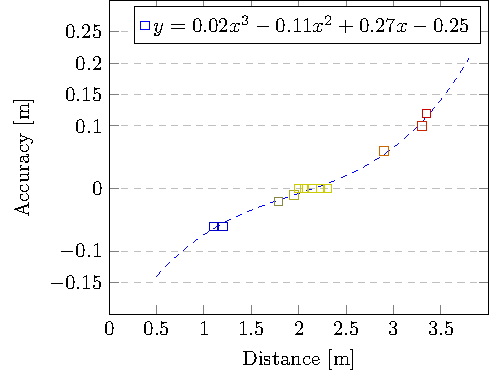
\includegraphics{Images/Fig06.pdf}
	\vspace{2.5cm}	
	\caption{Microsoft Kinect depth measurement accuracy by user distance}
	\label{fig:characteristics:kinect:distanceAccuracy}
\end{figure}
		
%=======================================================================		
\section{IMU characteristics}
IMU devices are in the professional usage for decades i.e. gyroscopes in rockets during II World War or in navigation systems in the aircrafts. Such devices became popular in home devices since they were implemented in MEMS architecture. In this article, all experiments were performed with the usage of IvenSense MPU-6050 module, which integrates accelerometer, gyroscope and thermometer on a single PCB. Both inertial sensors signals are affected by the external noise with different frequency characteristics and it needs to be filtered out to make these signals usable.

An accelerometer is a sensor responsible for a linear acceleration measurement in a form of the \textit{g-force}, so the device at  rest measures the force of $1g$ ($1g = 9.81\frac{m}{s^2}$) in upwards direction. However, accelerometer measures every single temporary force that works on this device and this is treated as a high frequency noise. That means, the filter used to remove such incorrect data must be one of the low pass filters. Also the technology used to build such sensor -- capacitive -- results in the sensitivity to operating temperature changes. Such influence was the subject of some scientists' researches \cite{Gebhardt2006,Grigorie1996}. The same influence was also observed in the used device, during the experiment, when the device measured g-force in the temperature range $10\degree C$ -- $50\degree C$. The results of  these measurements are presented in fig. \ref{fig:characteristics:imu:imuTemp}. If the IMU device is placed on a human body, its temperature rises up to approx. $30\degree C$, so it requires some sort of the compensation. The temperature model formula can be estimated according to eq. \eqref{eq:polynominal} as well.

The second inertial sensor -- a gyroscope -- measures the angular velocity in $deg/s$ units. Unlikely the accelerometer's short-term noise, the gyroscope suffers mostly from a constant, long-term bias that should be removed or limited. As this kind of noise is a low frequency signal, filter used to compensate it should be one of the high pass filters. This bias is also influenced by the operating temperature, however, there was no difference observed in filtered signals over the temperature range. It means that no additional compensation is required here.
 
In these types of devices we can also notice the incomplete information problem. The accelerometer, even though it measures forces along all 3 axes, allows us to calculate orientation around two of them only. The orientation (or the rotation) around the gravity vector is unmeasurable for such device. Theoretically, it is possible to calculate the orientation around all 3 axes with the gyroscope signal and its integration over the time. However, even the filtered signal contains some noise that grows rapidly due to the numerical integration and it quickly results in the significant drift that makes such measurements useless. Figure \ref{fig:characteristics:imu:gyroDrift} shows how noise affects the motion drift. During measurements, device was laying on table without any move, however, due to the uncompensated noise, estimation shows it has nominally rotated about $60\degree$.

\begin{figure}[h!]
	\centering 
	\begin{minipage}[b]{0.49\linewidth}
		\centering 
		%	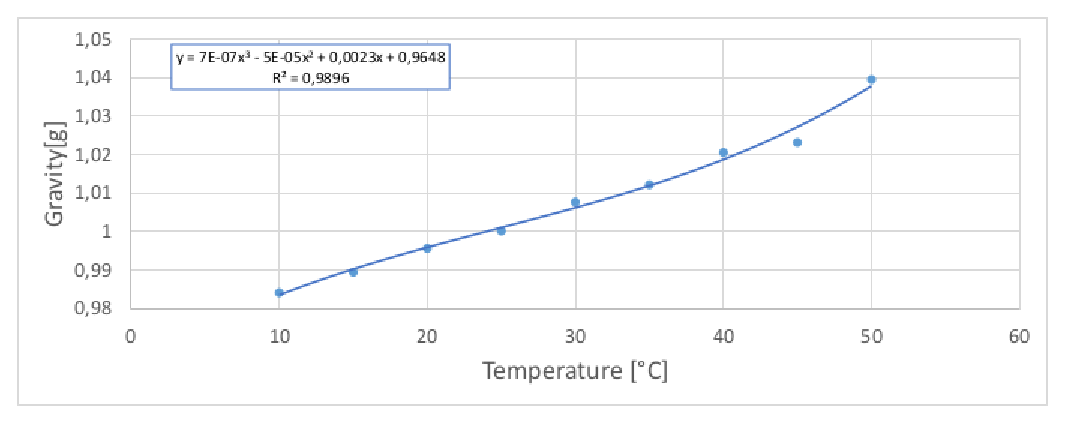
\includegraphics[width=0.95\textwidth]{Images/Fig07.eps}%{Images/Fig02.eps}
		\vspace{2.5cm}
		\caption{Gravity measurement in temperature range $10\degree C - 50\degree C$}
		\label{fig:characteristics:imu:imuTemp}
	\end{minipage}
	\begin{minipage}[b]{0.49\linewidth}
		\centering 
		%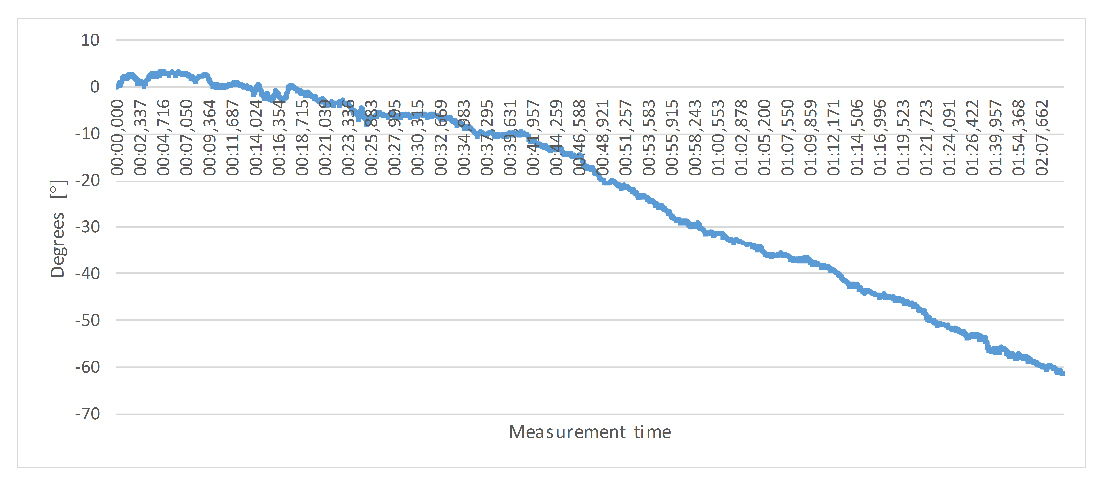
\includegraphics[width=0.95\textwidth]{Images/Fig08}%{Images/gyroDrift}
		\vspace{2.5cm}
		\caption{Gyroscope drift in non moved device}
		\label{fig:characteristics:imu:gyroDrift}
	\end{minipage}
\end{figure}

%===========================================================================
\section{Measurements imperfections compensation method}
\subsection{Kinect}
The compensation of Kinect measurements focuses on two aspects:
\begin{itemize}
	\item reducing the distance estimation inaccuracy according to the known model
	\item filtering unreliable joints positions estimations
\end{itemize}

The first aspect can be improved by the correction of the depth value (''$z$'' in Kinect's coordination space) by function $f(z)$ according to eq. \eqref{eq:characteristics:kinect:distanceCorrection} 

\begin{equation}
	z' = f(z) = -0.02*z^3 + 0.11*z^2 - 0.27*z + 0.25
	\label{eq:characteristics:kinect:distanceCorrection}
\end{equation}
where: $z'$ -- joint distance correction value.

This function is opposite to the function estimated from raw distance accuracy measurements, so adding it to the raw ''$z$'' value, reduces both: under- and overestimation.

The second problem -- unreliable measurements filtration -- can be reduced by the combination of few tools. First of all, joints positions should be filtered with the low pass filter (LPF). The Kinect camera works with the average frequency of $30Hz$ so rapid, extensive joint position changes between two consecutive frames is improbable. If such phenomena appears, LPF will remove such measurement. 

The other thing that should be taken into consideration is the user's orientation to the camera. From the experiments, which results are presented in fig. \ref{fig:characteristics:kinect:orientationCharts}, we can learn that the orientation greater than $50\degree$ cannot be considered as reliable measurement, so if Kinect is the only device used in the designed system, it is worth to consider some alert for the user to rotate back. Of course, the orientation angle calculation must be combined with ie. its variance in order to prevent ''false'' angles values (in fig. \ref{fig:characteristics:kinect:orientationCharts} the middle part of the chart shows values lower that $50\degree$, but with the significant fluctuation, which is typical for unreliable measurements). For correct values the standard deviation is close to 0, as there are no rapid changes in measurements (fig. \ref{fig:characteristics:imu:kinectRotationVariance}).

To summarize, decision if user's rotation to the Kinect is within reliable range takes into consideration following information:
\begin{itemize}
	\item both shoulders have tracking state set to \textsl{Tracked},
	\item orientation angle $\alpha$ is lower than $50\degree$,
	\item standard deviation of last 5 measured orientation angles is lower than $1.5\degree$.
\end{itemize}

\subsection{Inertial measurement unit}
The accelerometer and the gyroscope measurements are usually fused together in order to compensate the noise that affects both signals and to estimate the device orientation in the space. The most popular methods to achieve such fusion are Kalman filter \cite{Mccarron2013,Caron2006} and lately, Madgwick filter \cite{Kalkbrenner2014}. The accuracy comparison of these two filters can be found in the literature i.e. \cite{Madgwick2010}. Both of them can be described as a sort of complementary filters where two signals with low and high frequency noises are fused together with the proper noise reduction and some fusion factors. That allows to join together the same information from both sources with different level of importance. As the accelerometer signal needs to be filtered with LPF and its measurement is sensitive to the temperature, before it is fused with the gyroscope, the correction according to the temperature should be done. The regression analysis (eq. \eqref{eq:polynominal}) allowed to estimate the formula of accelerometer signal correction, described with eq. \eqref{eq:temperatureCompensation}. 

\begin{equation}
	\label{eq:temperatureCompensation}
	A' = \frac{A}{1+\beta(T - T_0)}
\end{equation}
where:
\begin{itemize}
	\item $A'$ -- corrected accelerometer measurement,
	\item $A$ -- accelerometer measurement,
	\item $T$ -- temperature measurement,
	\item $T_0$ -- device reference operating temperature. For used device $T_0 = 25\degree C$,
	\item $\beta$ -- correction factor. For used device $\beta = 0.0011$.
\end{itemize}

The results of such correction, influenced by different $\beta$ is presented in figure~\ref{fig:characteristics:imu:imuTempCompensation}. Parameter $\beta$ has been estimated on sample measurements analysis and chosen based on average error between expected and actual values in each measurement point. Next, these signals can be used in the fusion filter. 

\begin{figure}[h!]
	\centering 
	%	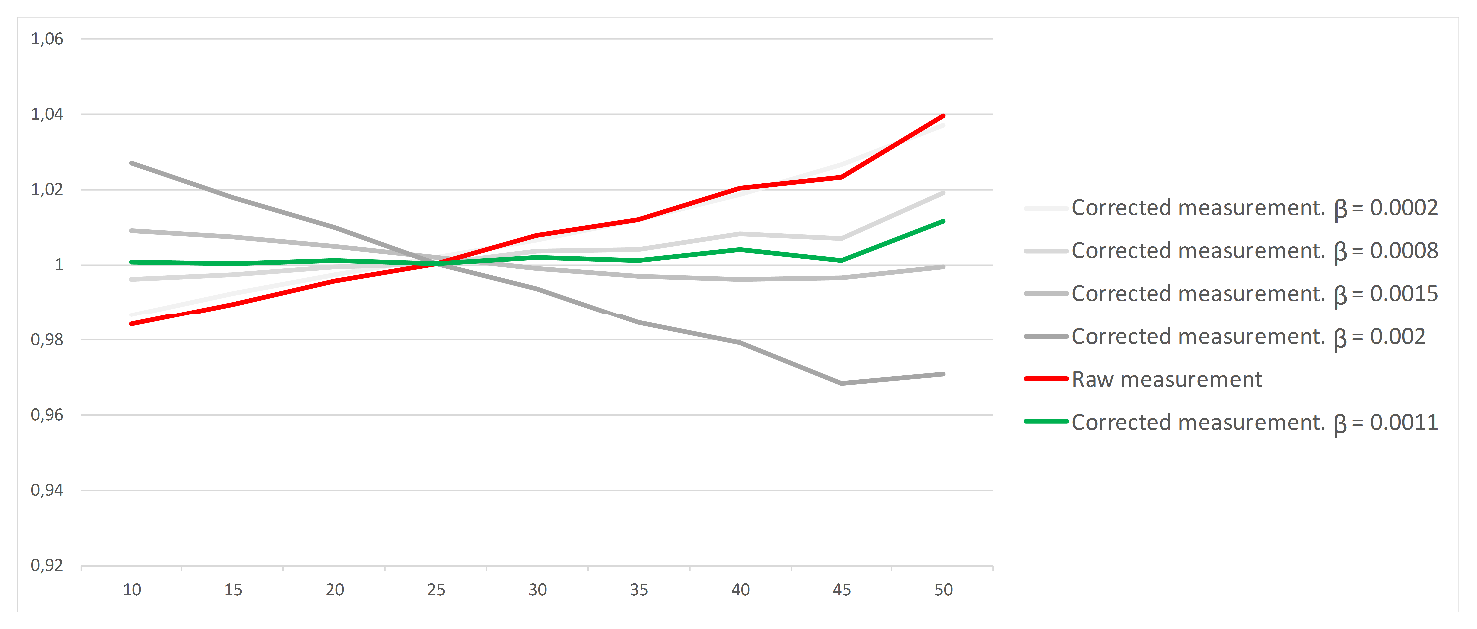
\includegraphics[width=0.65\textwidth]{Images/Fig09}%{Images/temperaure}
	\vspace{2.5cm}
	\caption{Gravity measurement compensation due to the temperature and $\beta$ factor.}
	\label{fig:characteristics:imu:imuTempCompensation}
\end{figure}

\subsection{Information incompleteness correction}
Compensation methods presented previously are able to improve the quality of data gathered from both types of devices, however, are not able to add the missing information about rotations (Kinect -- roll -- rotation along the bone; IMU -- yaw -- rotation around gravity vector). To achieve that, both signals: from Kinect and IMU must be fused together. Then, the combined data will include full set of information. In the literature there are presented several methods of Kinect and IMU data fusion \cite{Tian2015,Bo2011,Kalkbrenner2014} and each of them has different approach to such fusion and the different accuracy (Kalkbrener \cite{Kalkbrenner2014} declared standard deviation of the joint coordinates measurements of $\pm2.20cm$ for \textit{face off} trunk position). To verify influence of flaws described in this article, series of experiments has been performed with algorithm proposed by Kalkbrenner and implemented according to published description. Results returned by this implementation had slightly different accuracy than declared and they differed for both joints: $\pm2.90cm$ for elbow and  $\pm3.60cm$ for wrist. Then, original method has been modified by adding IMU temperature and Kinect distance corrections as well as decreasing importance of Kinect measurements if user was considerably rotated to the camera. 

Methods have been tested on a set of four upper limbs moves that are presented in fig. \ref{fig:poses}. Each move sequence (repeated 5 times) started in \textsl{T-pose} and ended up in one of the final pose presented in mentioned picture. 

\begin{figure}[h!]
	\centering
	%	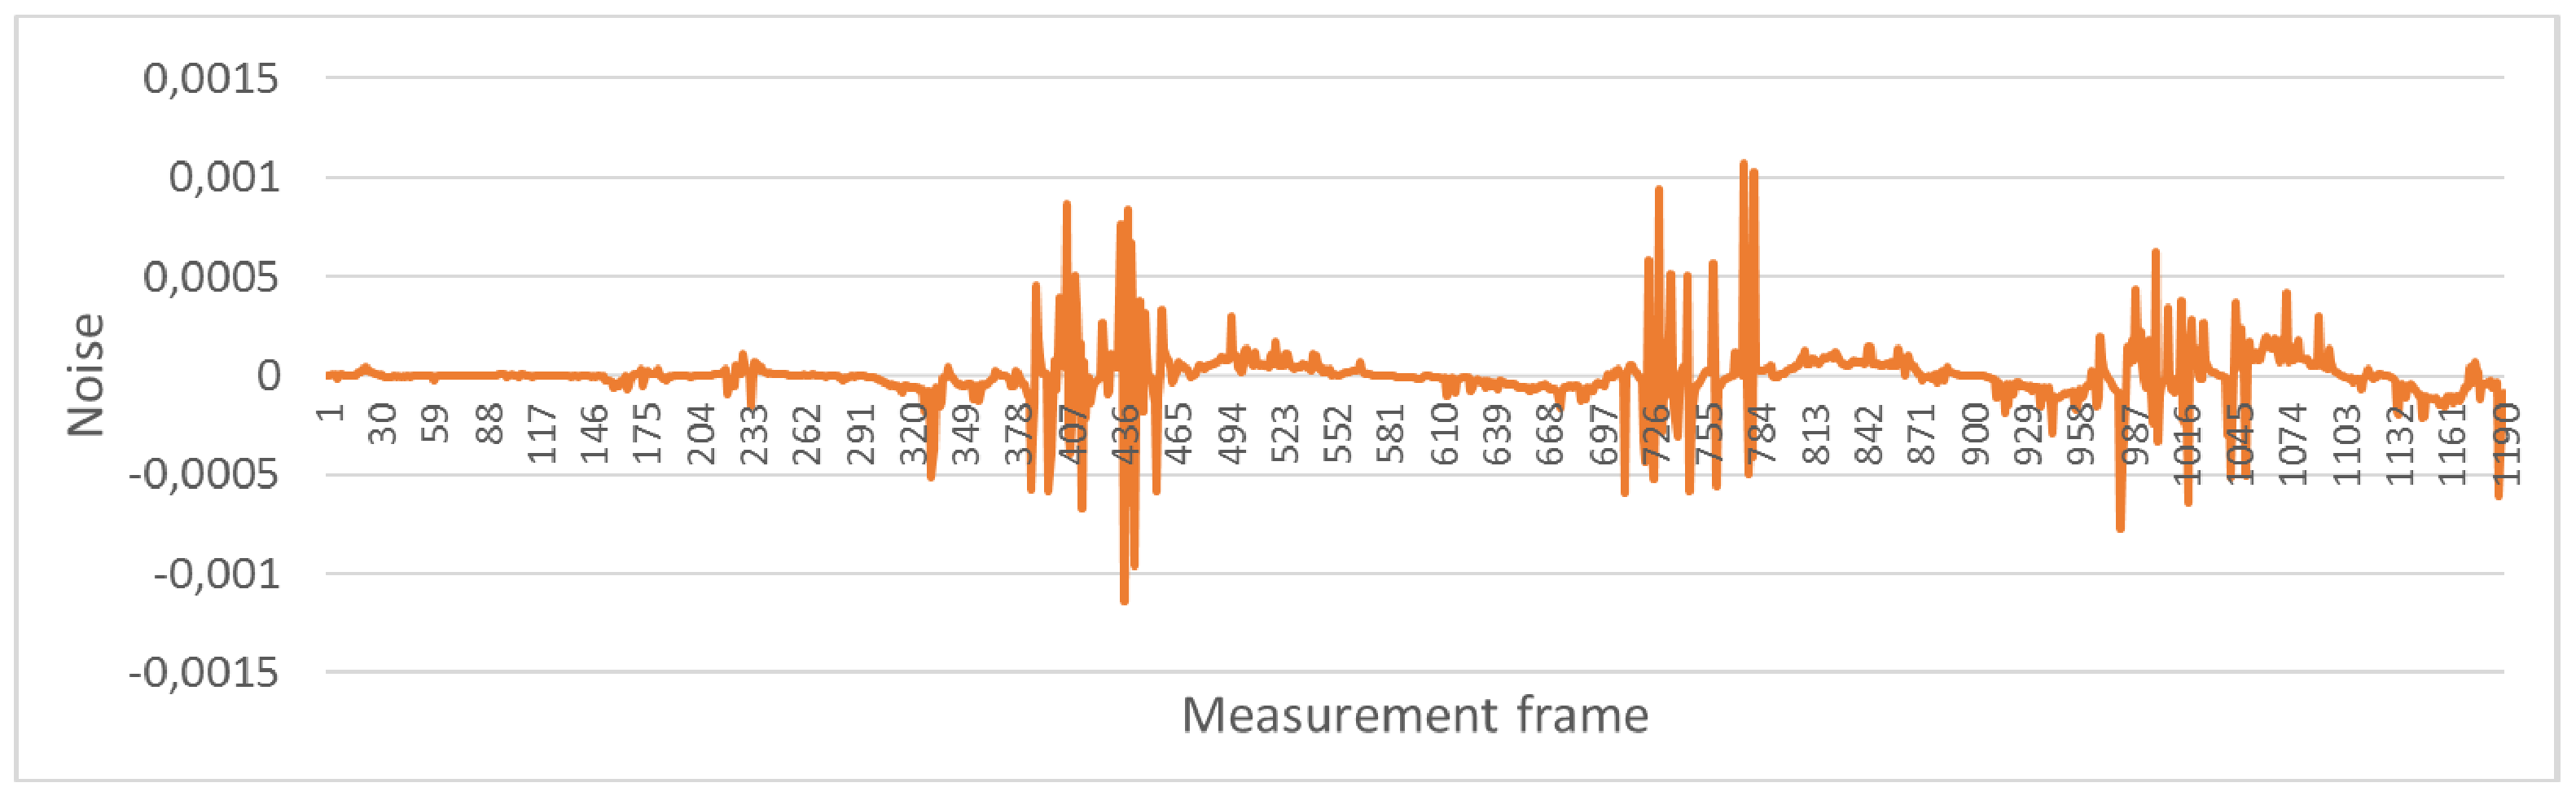
\includegraphics[width=0.35\textwidth]{images/Fig10.eps}%{images/Fig12.eps}
	\vspace{2.5cm}
	\caption{Movement sequences performed during tests.}
	\label{fig:poses}
\end{figure}

Average improvement of joints positioning accuracy has been noticed for about $12\%$. Comparison of results of both methods has been presented in table~\ref{tab:summary} and in figures \ref{fig:positionElbow} and \ref{fig:positionWrist}. 

\begin{table}[]
	\centering
		
	\caption{Summarized results accuracy for original and corrected Kalkbrenner methods}
	\label{tab:summary}
	\begin{tabular}{l|l|l|l|l|}
		\cline{2-5}
		                                & \multicolumn{1}{c|}{Elbow} & \multicolumn{1}{c|}{Elbow corrected} & \multicolumn{1}{c|}{Wrist} & \multicolumn{1}{c|}{Wrist corrected} \\ \hline
		\multicolumn{1}{|l|}{Average}   & 0.029                      & 0.026                                & 0.036                      & 0.032                                \\ \hline
		\multicolumn{1}{|l|}{Std. dev.} & 0.006                      & 0.005                                & 0.01                       & 0.009                                \\ \hline
	\end{tabular}
	
\end{table}

\begin{figure}[h!]
	\centering
	\begin{minipage}[b]{0.49\linewidth}
		\centering   
		%	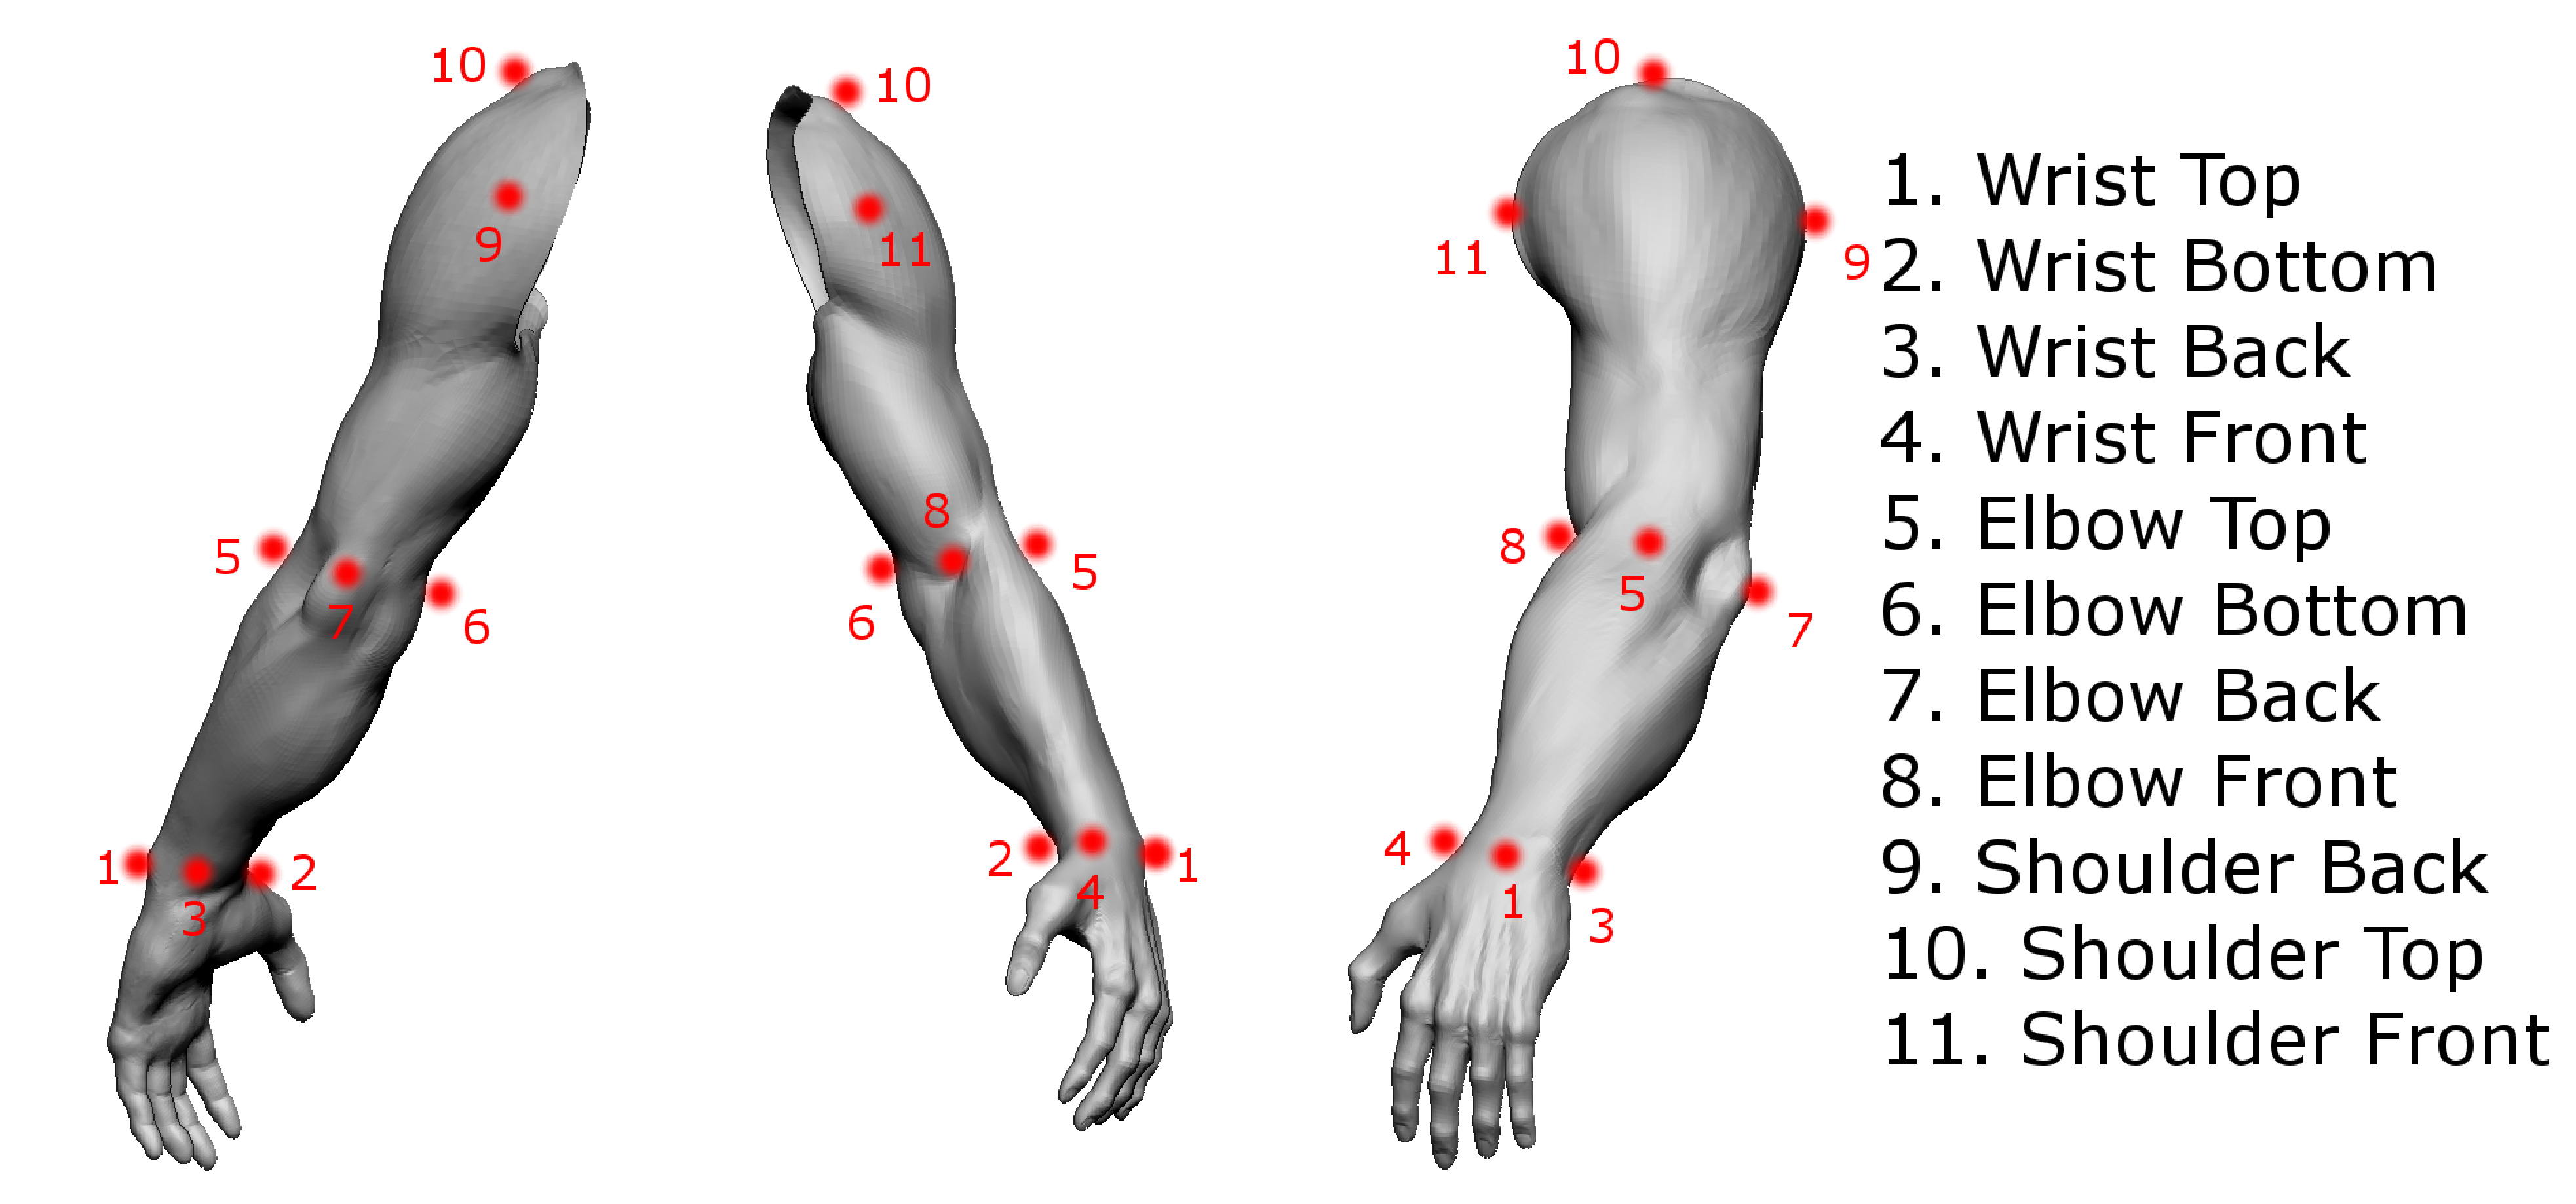
\includegraphics[width=\textwidth]{images/Fig11}%{images/elbow}
		\vspace{2.5cm}
		\caption{Elbow positioning average accuracy}
		\label{fig:positionElbow}
	\end{minipage}
	\begin{minipage}[b]{0.49\linewidth}
		\centering 
		%	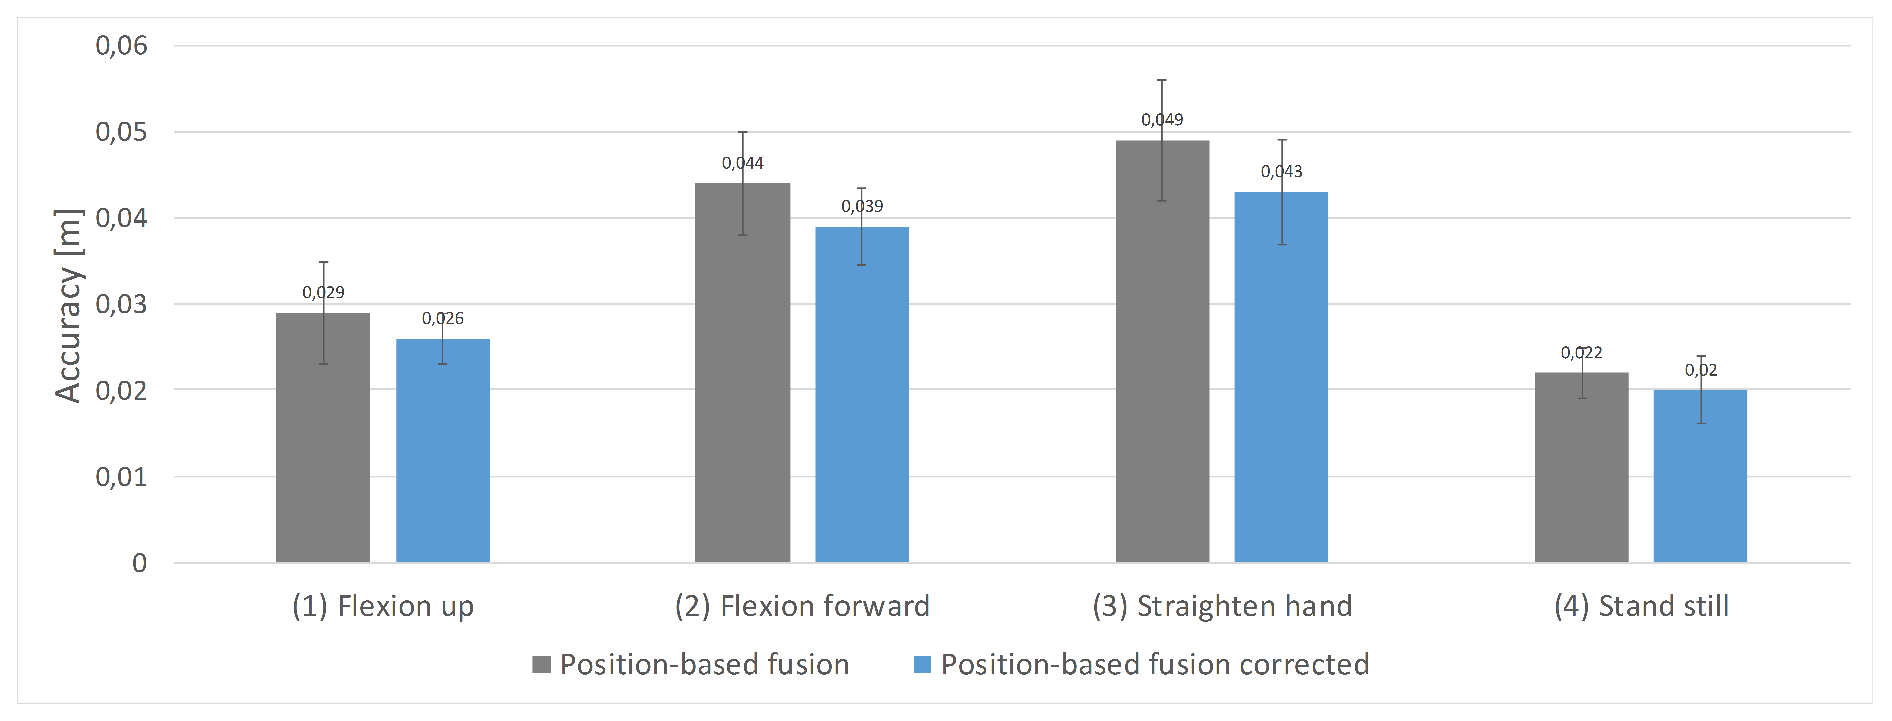
\includegraphics[width=\textwidth]{images/Fig12}%{images/wrist}
		%vspace{2.5cm}
		\caption{Wrist positioning average accuracy}
		\label{fig:positionWrist}
	\end{minipage}
				
\end{figure}
%=============================================================		
\section{Summary}
In this paper authors presented the analysis of two popular motion tracking devices characteristics. Authors elaborated a new method of measurements imprecision and limitations compensation, respecting characteristics of considered devices. The method respected compensation of data flaws for each device individually, as well as data streams fusion. It has provided set of estimated sensors characteristics that were originally missing in the individual devices. Aggregated, human limbs tracking, device challenging, experiments have revealed considerable, about 12\%, increase in considered joints tracking accuracy.
%Also the new,  original Kinect and IMU fusion method that includes compensation of pointed devices' imperfections has been presented.

		
\begin{thebibliography}{5}
	
		
	\bibitem{Asteriadis2013}
	Asteriadis, S. , et al.:
	Estimating human motion from multiple Kinect sensors.
	Proc. 6th Int. Conf. Comput. Vis. / Comput. Graph. Collab. Tech. Appl. - MIRAGE '13 (2013)
			
	\bibitem {Bo2011}
	Bo, Antonio Padilha Lanari et al:
	Joint angle estimation in rehabilitation with inertial sensors and its integration with Kinect.
	Proc. of the Ann. Int. Conf. of the IEEE Eng. in Med. and Bio. Soc., EMBS/2011 (2011)
			
	\bibitem {Caron2006}	
	F. Caron F., et al.: 
	GPS/IMU data fusion using multisensor Kalman filtering: introduction of contextual aspects. 
	Inf. Fusion, pp. 221–230, (2006).
				
	\bibitem {Chang2011}
	Chang, Y.-J., et al.:
	A Kinect-based system for physical rehabilitation: a pilot study for young adults with motor disabilities.
	Res. Dev. Disabil., vol. 32, no. 6, pp. 2566–70, Dec. 2011.
				
	\bibitem {Destelle2014}
	Destelle, F., et al.: Low-cost accurate skeleton tracking based on fusion of kinect and wearable inertial sensors,
	Proc. of the 22nd Euro. IEEE Sig. Proc. Conf. (EUSIPCO), p. 371-375 (2014)
	
	\bibitem{DiFilippo2015}
	DiFilippo, N. M. and Jouaneh, M. K.:
	Characterization of Different Microsoft Kinect Sensor Models.
	IEEE Sensors Journal, vol 15, 8, 4554-4564 (2015)
				
	\bibitem{Fofi2004}
	Fofi, D and Sliwa, T and Voisin, Y:
	A comparative survey on invisible structured light.
	SPIE Electron. Imaging Machine Vis. Appl. Ind. Insp. XII San Jos{\'{e}} USA (2004)
				
	\bibitem{patent:20100118123}
	Freedman, B., et al.:
	Depth Mapping Using Projected Patterns.
	Patent:20100118123
	%Available: \url{http://www.freepatentsonline.com/y2010/0118123.html} [Accessed: 12-Apr-2016]
				
	\bibitem {Gebhardt2006}
	S. Gebhardt, G. Scheinert, and F. H. Uhlmann:
	Temperature influence on capacitive sensor structures.
	Inf. tech. and electrical eng. - dev. and sys., materials and tech. for the future, (2006)
		
	\bibitem{Glonek2016}
	Glonek, G. and Wojciechowski, A.:
	Hybrid method of human limb joints positioning -- hand movement case study.
	Proc. 5th Int. Conf. Info. Tech. in Biomed. (2016) [In press]
		
	\bibitem {Grigorie1996}
	M. Grigorie, C. de Raad, F. Krummenacher, and C. Enz:
	Analog Temperature Compensation for Capacitive Sensor Interfaces (1996).
			
	\bibitem {Jayalath2013}
	Jayalath, S. and  Murray, I.: 
	A Gyroscope Based Accurate Pedometer Algorithm.
	Int. Conf. Indoor Position. Indoor Navig., no. October, p. 31, (2013).
			
	\bibitem {kinectFixit2016}
	iFixIt:
	Xbox 360 Kinect Teardown - iFixit.
	Available: \url{https://www.ifixit.com/Teardown/Xbox+360+Kinect+Teardown/4066} [Accessed: 12-Apr-2016]
	
	\bibitem {Kalkbrenner2014}
	Kalkbrenner, Christoph et al:
	Motion Capturing with Inertial Measurement Units and Kinect - Tracking of Limb Movement using Optical and Orientation Information.
	Proc. of the Int. Conf. on Biomed. Electro. and Dev. (2014)
				
	\bibitem{Kitsikidis2011}
	Kitsikidis, A. , et al.:
	Dance Analysis using Multiple Kinect Sensors (2011).
	
	\bibitem{Lange2012}
	Lange, B., et al.: 
	Interactive game-based rehabilitation using the Microsoft Kinect,
	2012 IEEE Virtual Real., pp. 171–172, Mar. (2012).
	
	\bibitem {Madgwick2010}
	Madgwick, S.O.H.:
	An efficient orientation filter for inertial and inertial/magnetic sensor arrays. (2010)
		
	\bibitem {Mccarron2013}		
	Mccarron, B. :
	Low-Cost IMU Implementation via Sensor Fusion Algorithms in the Arduino Environment (2013)
				
	\bibitem {Murray-Smith2014}
	Feng, S. and Murray-Smith, R.: Fusing Kinect Sensor and Inertial Sensors with Multi-rate Kalman Filter.
	IET Conf. Data Fusion Target Track. 2014 Algorithms Appl. (2014)
	
	\bibitem{reichinger2011}
	Reichinger, A.:
	Kinect Pattern Uncovered.
	Available: \url{https://azttm.wordpress.com/} [Accessed: 12-Apr-2016]
				
	\bibitem{Rzeszotarski2006}
	Rzeszotarski, D and Strumi{\l}{\l}o, P., et al.:
	System Obrazowania Stereoskopowego Sekwencji Scen Tr{\'{o}}jwymiarowych.
	Zesz. Nauk. Elektron. (2006)
	
	\bibitem{Schroder2011}
	Schr{\"{o}}der, Y. , et al.:
	Multiple Kinect Studies Technical Report (2011).
			
	\bibitem{Shotton2008}
	Shotton, J. , et al.:
	Semantic Texton Forests for Image Categorization and Segmentation.		
	Proc. IEEE CVPR (2008)		
			
	\bibitem{Shotton2011}
	Shotton, J. , et al.:
	Real-time human pose recognition in parts from single depth images.		
	Proc. IEEE CVPR (2011)	
					
	\bibitem{patent:20080106746}
	Shpunt, A. and Zalevsky, Z.:
	Depth-varying light fields for three dimensional sensing.
	Patent:20080106746
	%Available: \url{http://www.freepatentsonline.com/y2008/0106746.html} [Accessed: 12-Apr-2016]
					
	\bibitem{patent:20100020078}
	Shpunt, A.:
	Depth Mapping Using Multi-Beam Illumination.
	Patent:20100020078
	%	Available: \url{http://www.freepatentsonline.com/y2010/0020078.html} [Accessed: 12-Apr-2016]
	
	\bibitem{stack:kinect2011}
	Stackoverflow Community:
	Precision of the kinect depth camera.[Accessed: 12-Apr-2016]
	%Available: \url{http://stackoverflow.com/questions/7696436/precision-of-the-kinect-depth-camera} 
	
	\bibitem{Suarez2012}
	Suarez, J. and Murphy, R. R.:
	Using the Kinect for search and rescue robotics.
	2012 IEEE Int. Symp. on Safety, Security, and Rescue Robotics (SSRR) (2012)
				
	\bibitem{Tian2015}
	Tian, Yushuang et al:
	Upper limb motion tracking with the integration of IMU and Kinect
	Neurocomputing (2015)
		
	\bibitem{walklogger}
	Walklogger:
	Available: \url{https://play.google.com/store/apps/details?id=com.walklogger.pedometer} [Accessed: 17-Apr-2016]
		
\end{thebibliography}
\end{document}